\documentclass[12pt]{article}
\usepackage[utf8]{inputenc}

\usepackage{lmodern}

\usepackage{enumitem}
\usepackage[margin=2cm]{geometry}

\usepackage{amsmath, amsfonts, amssymb}
\usepackage{graphicx}
%\usepackage{subfigure}
\usepackage{tikz}
\usepackage{pgfplots}
\usepackage{multicol}

\usepackage{comment}
\usepackage{url}
\usepackage{calc}
\usepackage{subcaption}
\usepackage[indent=0pt]{parskip}
\usepackage{animate}

\usepackage{array}
\usepackage{blkarray,booktabs, bigstrut}
\usepackage{bigints}

\pgfplotsset{compat=1.16}

% MATH commands
\newcommand{\ga}{\left\langle}
\newcommand{\da}{\right\rangle}
\newcommand{\oa}{\left\lbrace}
\newcommand{\fa}{\right\rbrace}
\newcommand{\oc}{\left[}
\newcommand{\fc}{\right]}
\newcommand{\op}{\left(}
\newcommand{\fp}{\right)}

\newcommand{\bi}{\mathbf{i}}
\newcommand{\bj}{\mathbf{j}}
\newcommand{\bk}{\mathbf{k}}
\newcommand{\bF}{\mathbf{F}}

\newcommand{\mR}{\mathbb{R}}

\newcommand{\ra}{\rightarrow}
\newcommand{\Ra}{\Rightarrow}

\newcommand{\sech}{\mathrm{sech}\,}
\newcommand{\csch}{\mathrm{csch}\,}
\newcommand{\curl}{\mathrm{curl}\,}
\newcommand{\dive}{\mathrm{div}\,}

\newcommand{\ve}{\varepsilon}
\newcommand{\spc}{\vspace*{0.5cm}}

\DeclareMathOperator{\Ran}{Ran}
\DeclareMathOperator{\Dom}{Dom}

\newcommand{\exo}[1]{\noindent\textcolor{red}{\fbox{\textbf{Problem {#1}}}\hrulefill}\\}
\newcommand{\qu}[4]{\noindent\textcolor{#4}{\fbox{\textbf{Section {#1} | Problem {#2}}} \hrulefill{{\fbox{\textbf{{#3} Points}}}}\\}}

\newcommand{\semester}{Spring 2023}

\newcommand{\CVup}{%

\begin{tikzpicture}
\draw[black, <->, >=latex] (-0.33, 0.5) .. controls (-0.125, 0) and (0.125, 0) .. (0.33, 0.5);
\end{tikzpicture}}

\newcommand{\CVupInc}{%
\begin{tikzpicture}
\draw[black, ->, >=latex] (0,0) .. controls (0.2, 0) and (0.4, 0.2) .. (0.5, 0.5);
\end{tikzpicture}}

\newcommand{\CVupDec}{%
\begin{tikzpicture}[rotate=270]
\draw[black, ->, >=latex] (0,0) .. controls (0.2, 0) and (0.4, 0.2) .. (0.5, 0.5);
\end{tikzpicture}}

\newcommand{\CVdown}{%
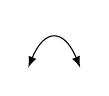
\begin{tikzpicture}
\draw[black, <->, >=latex] (-0.33, -0.5) .. controls (-0.125, 0) and (0.125, 0) .. (0.33, -0.5);
\end{tikzpicture}}

\newcommand{\CVdownInc}{%
\begin{tikzpicture}
\draw[black, ->, >=latex] (-0.5, -0.5) .. controls (-0.5, -0.3) and (-0.5, -0.1) .. (0,0);
\end{tikzpicture}}

\newcommand{\CVdownDec}{%
\begin{tikzpicture}[rotate=-90]
\draw[black, ->, >=latex] (-0.5, -0.5) .. controls (-0.5, -0.3) and (-0.5, -0.1) .. (0,0);
\end{tikzpicture}}

\begin{document}
	\noindent \hrulefill \\
	MATH-241 \hfill Pierre-Olivier Paris{\'e}\\
	Solutions Section 1-5 \hfill \semester \\\vspace*{-1cm}
	
	\noindent\hrulefill
	
	\spc
	
	\exo{4}
	
	\begin{enumerate}
	\item[(a)] $\lim_{x \ra 2^-} f(x) = 3$.
	\item[(b)] $\lim_{x \ra 2^+} f(x) = 1$.
	\item[(c)] $\lim_{x \ra 2}$ doesn't exist because the limit on the left is different from the limit on the right.
	\item[(d)] $f(2) = 3$.
	\item[(e)] $\lim_{x \ra 4} f(x) = 4$ because the limit from the left and the limit from the right are $4$.
	\item[(f)] $f(4)$ doesn't exist. 
	\end{enumerate}
	
	\spc
	
	\exo{16}
	\\
	Here is a graph that satisfies the requirementss.
	
	\begin{figure}[h!]
	\centering
	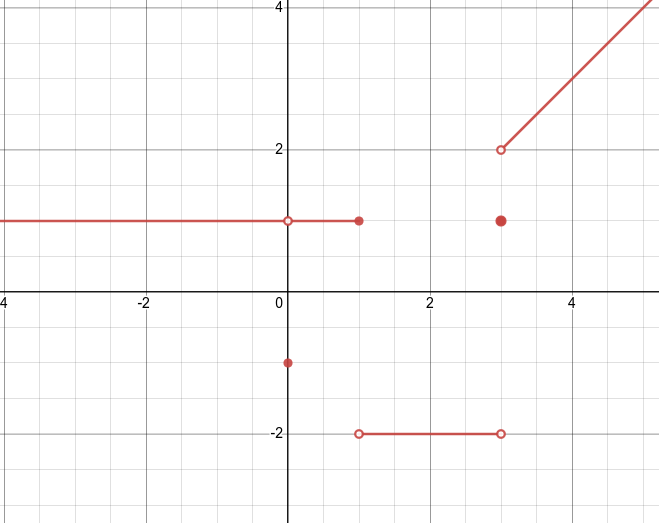
\includegraphics[scale=0.5]{fig_1.png}
	\caption{Graph of the function $f$}
	\end{figure}
	
	We see from the graph that
		\begin{itemize}
		\item $f(0) = -1$ and $f(3) = 1$;
		\item $\lim_{x \ra 0} f(x) = 1$;
		\item $\lim_{x \ra 3^-} f(x) = -2$;
		\item $\lim_{x \ra 3^+} f(x) = 2$.
		\end{itemize}
	
	\spc

	\exo{22}
	\\
	We build a table
	\begin{center}
		\begin{tabular}{c|c}
		$x$ & $f(x)$ \\ \hline
0.500000 & 131.312500 \\  \hline
0.100000 & 88.410100 \\ \hline
0.010000 & 80.804010 \\ \hline
0.001000 & 80.080040 \\ \hline
0.000100 & 80.008000 \\ \hline
-0.500000 & 48.812500 \\ \hline
-0.100000 & 72.390100 \\ \hline
-0.010000 & 79.203990 \\ \hline
-0.001000 & 79.920040 \\ \hline
-0.000100 & 79.992000 \\ 
		\end{tabular}
	\end{center}
	
	We can guess from the values from the table that
		\begin{align*}
		\lim_{h \ra 0} \frac{(2 + h)^5 - 32}{h} = 80 .
		\end{align*}
		
	\spc
	
	\exo{30}
	\\
	We see that the limit on the numerator is $6$ and the limit of the denominator is $0^-$ meaning that the value approaches $0$ from the left. So we have a number divided by a very small negative quantity. We then get
		\begin{align*}
		\lim_{x \ra 5^-} \frac{x + 1}{x - 5} = 6 / 0^- = -\infty .
		\end{align*}
	
	\spc
	
	\exo{34}
	\\
	As $x$ approaches $0^-$ (so $x$ approaches $0$ from the left), then $x - 1$ approaches $-1^-$ (so a number closed to $-1$ from the left) and $x + 2$ approaches $2^-$ (so a number closed to $2$ from the left). Therefore, the quotient $(x - 1)/(x^2 (x + 2))$ approaches $-1^- / (0^-)^2 (2^-) = -\infty$ because we divided by the square of a small negative number (really really close to zero, but negative) which turns out to be a small positive number.
	
	As $x$ approaches $0^+$ (so $x$ approaches $0$ from the right), then $x-1$ approaches $-1^+$ (so a number closed to $-1$ from the right) and $x + 2$ approaches $2^+$ (so a number closed to $2$ from the left). Therefore, the quotient $(x - 1)/(x^2 (x + 2))$ approaches $-1^+ / (0^+ 2^+) = -\infty$ because we divided by the square of a small positive number (really really close to zero, but positive) which turns out to be a small positive number.
	
	Therefore, from the above observations, we conclude that
		\begin{align*}
		\lim_{x \ra 0^-} \frac{x - 1}{x^2 (x + 2)} = \lim_{x \ra 0^+} \frac{x -1}{x^2 (x +2)} = -\infty .
		\end{align*}
	
	\spc
	
	\exo{38}
	\\
	First, we notice that
		\begin{align*}
		\frac{x^2 - 2x}{x^2 - 4x + 4} = \frac{x(x - 2)}{(x -2 )^2} = \frac{x}{(x - 2)} .
		\end{align*}
	Therefore, we see that, as $x$ approaches $2$ from the left, $x - 2$ will be a small negative number (approaching $0$ from the left) and $x$ will approach $2$. Therefore, 
		\begin{align*}
		\lim_{x \ra 2^-} \frac{x}{x - 2} = \frac{2}{0^-} = -\infty .
		\end{align*}
		

\end{document}